%%%%%%%%%%%%%%%%%%%%%%%%%%%%%%%%%%%%%%%%%%%%%%%%%%%%%%
% A Beamer template for University of Wollongong     %
% Based on THU beamer theme                          %
% Author: Qiuyu Lu                                   %
% Date: July 2024                                    %
% LPPL Licensed.                                     %
%%%%%%%%%%%%%%%%%%%%%%%%%%%%%%%%%%%%%%%%%%%%%%%%%%%%%%
% Customized for Sharif University of Technology     %
%%%%%%%%%%%%%%%%%%%%%%%%%%%%%%%%%%%%%%%%%%%%%%%%%%%%%%


\documentclass[serif, aspectratio=169]{beamer}
%\documentclass[serif]{beamer}  % for 4:3 ratio
\usepackage[T1]{fontenc} 
\usepackage{fourier} % see "http://faq.ktug.org/wiki/uploads/MathFonts.pdf" for other options
\usepackage{hyperref}
\usepackage{latexsym,amsmath,xcolor,multicol,booktabs,calligra}
\usepackage{graphicx,pstricks,listings,stackengine}
\usepackage{lipsum}
\usepackage{ragged2e}
\usepackage{colortbl}
\usepackage{times}
\usepackage{fancyhdr,graphicx,amsmath,amssymb,algorithm,algpseudocode,mathtools,needspace}
\usepackage{tikz}
    \usetikzlibrary{positioning}
% For writing comments that are aligned to the left side
\makeatletter
\NewDocumentCommand{\LeftComment}{s m}{%
  \Statex \IfBooleanF{#1}{\hspace*{\ALG@thistlm}}\(\triangleright\) #2}
\makeatother
% To manually indent states in algorithmicx
\newcommand{\IndState}{\State\hspace{\algorithmicindent}}
% To make breakable algorithms
\makeatletter
\newenvironment{nofloatalgorithmic}[2][0]
  {
  \par
  \needspace{\dimexpr\baselineskip+6.8pt}
  \noindent
  \hrule height.8pt depth0pt \kern2pt
  \refstepcounter{algorithm}
  \addcontentsline{loa}{algorithm}{\numberline{\thealgorithm}#2}
  \noindent\textbf{\fname@algorithm~\thealgorithm} #2\par
  \kern2pt\hrule\kern2pt
  \begin{algorithmic}[#1]
  }
  {
  \end{algorithmic}
  \nobreak\kern2pt\hrule\relax
  }
\makeatother
% To make vertical arrow
\newcommand\vertarrowbox[3][6ex]{%
  \begin{array}[t]{@{}c@{}} #2 \\
  \left\uparrow\vcenter{\hrule height #1}\right.\kern-\nulldelimiterspace\\
  \makebox[0pt]{\scriptsize#3}
  \end{array}%
}
\DeclareMathOperator*{\argmax}{argmax}

\author{Ali Sharifi-Zarchi}
\title{Machine Learning (CE 40717)}
\subtitle{Fall 2025}
\institute{
    CE Department \\
    Sharif University of Technology
}
%\date{\small \today}
% \usepackage{UoWstyle}
\usepackage{SUTstyle}

% defs
\def\cmd#1{\texttt{\color{red}\footnotesize $\backslash$#1}}
\def\env#1{\texttt{\color{blue}\footnotesize #1}}
\definecolor{deepblue}{rgb}{0,0,0.5}
\definecolor{deepred}{RGB}{153,0,0}
\definecolor{deepgreen}{rgb}{0,0.5,0}
\definecolor{halfgray}{gray}{0.55}

\lstset{
    basicstyle=\ttfamily\small,
    keywordstyle=\bfseries\color{deepblue},
    emphstyle=\ttfamily\color{deepred},    % Custom highlighting style
    stringstyle=\color{deepgreen},
    numbers=left,
    numberstyle=\small\color{halfgray},
    rulesepcolor=\color{red!20!green!20!blue!20},
    frame=shadowbox,
}




\begin{document}

\begin{frame}
    \titlepage
    \vspace*{-0.6cm}
    \begin{figure}[htpb]
        \begin{center}
            
\includegraphics[keepaspectratio, scale=0.1]{pic/sharif-main-logo.png}
        \end{center}
    \end{figure}
\end{frame}

\begin{frame}
\tableofcontents[sectionstyle=show,
subsectionstyle=show/shaded/hide,
subsubsectionstyle=show/shaded/hide]
\end{frame}

\section{Performance metrics}

\begin{frame}{Evaluation Context}
    \begin{itemize}
        \item Model evaluation quantifies predictive performance on unseen data.
        \item Metrics are derived from the confusion matrix:
    \end{itemize}
    \vspace{0.3cm}
    \begin{center}
    \begin{tabular}{c|cc}
        \toprule
        & Predicted Positive & Predicted Negative \\
        \midrule
        Actual Positive & TP & FN \\
        Actual Negative & FP & TN \\
        \bottomrule
    \end{tabular}
    \end{center}
    \vspace{0.3cm}
    \begin{itemize}
        \item TP, TN, FP, FN provide the foundation for classification performance indices.
    \end{itemize}
\end{frame}

\begin{frame}{Accuracy in classification problems}
    \begin{itemize}
        \item \textbf{Accuracy} is one of the simplest and most commonly used performance metrics.
        \item It is defined as the ratio of correctly predicted instances to the total instances:
        \[
        \text{Accuracy} = \frac{\text{True Positives} + \text{True Negatives}}{\text{Total Samples}}
        \]
        \textbf{Error Rate:} complement of accuracy
        \[
        \text{Error Rate} = \frac{FP + FN}{TP + TN + FP + FN} = 1 - \text{Accuracy}
    \]
        \item However, accuracy alone can be misleading, especially with imbalanced datasets.
    \end{itemize}
\end{frame}

\begin{frame}{Example: cancer detection problem}
    \begin{itemize}
        \item Imagine a dataset with 1000 patients:
        \begin{itemize}
            \item Only 10 have cancer (\textbf{positive class}).
            \item 990 do not have cancer (\textbf{negative class}).
        \end{itemize}
        \item A classifier predicts that no one has cancer (predicts all as negative).
        \item What will be the accuracy of this model?
    \end{itemize}
\end{frame}

\begin{frame}{Example: cancer detection problem cont.}
    Look at this table for our model which predict negative all the time:
    
    \begin{table}[h!]
        \centering
        \begin{tabular}{@{}lcc@{}}
            \toprule
            & \textbf{Predicted Negative} & \textbf{Predicted Positive} \\ \midrule
            \textbf{Actual Negative} & 990 (TN) & 0 (FP) \\
            \textbf{Actual Positive} & 10 (FN)  & 0 (TP) \\ \bottomrule
        \end{tabular}
        % \caption*{Confusion Matrix for Cancer Detection (All Negative Predictions)}
    \end{table}
    
    \[
    \text{Accuracy} = \frac{990 + 0}{1000} = 99\%
    \]
    
    \textbf{High accuracy}, but the model fails to detect any actual cases of cancer!
\end{frame}


\begin{frame}{Why accuracy can be misleading}
    \begin{itemize}
        \item In highly imbalanced datasets (e.g., cancer detection), the \textbf{minority class} (positive cases) is often underrepresented.
        \item A model that always predicts the majority class can still have high accuracy, but poor real-world performance.
        \item In the cancer detection example, 99\% accuracy sounds good, but the model doesn't detect any actual cancer cases.
        \item We need better metrics to evaluate model performance.
    \end{itemize}
\end{frame}
%%%%%%%%%%%%%%%%%%%%%%%%%%%%%%%%%%%%%%%%%%%%%%%%
\begin{frame}{Performance metrics}
    \begin{itemize}
        \item \textbf{Scenario:}
        \begin{itemize}
            \item An alarm system can either ring or not ring when a thief is present.
            \item Let's define the outcomes:
            \begin{itemize}
                \item \textbf{True Positive (TP)}: Alarm rings (correctly) when a thief is present.
                \item \textbf{True Negative (TN)}: Alarm does not ring (correctly) when no thief is present.
                \item \textbf{False Positive (FP)}: Alarm rings (incorrectly) when no thief is present (a false alarm).
                \item \textbf{False Negative (FN)}: Alarm does not ring (incorrectly) when a thief is present (a missed alarm).
            \end{itemize}
        \end{itemize}
    \end{itemize}
    
    % \begin{table}[h!]
    %     \centering
    %     \begin{tabular}{@{}lcc@{}}
    %         \toprule
    %         & \textbf{Thief Present} & \textbf{No Thief Present} \\ \midrule
    %         \textbf{Alarm Rings} & TP & FP \\
    %         \textbf{Alarm Does Not Ring} & FN & TN \\ \bottomrule
    %     \end{tabular}
    %     % \caption*{Confusion Matrix for Alarm System}
    % \end{table}
    
    \begin{minipage}{0.7\textwidth} % Left side for the table
        \begin{table}[h!]
            \centering
            \begin{tabular}{@{}lcc@{}}
                \toprule
                & \textbf{Thief Present} & \textbf{No Thief Present} \\ \midrule
                \textbf{Alarm Rings} & TP & FP \\
                \textbf{Alarm Does Not Ring} & FN & TN \\ \bottomrule
            \end{tabular}
        \end{table}
        
        
    \end{minipage}\hfill 
    \begin{minipage}{0.2\textwidth} 
        \centering
        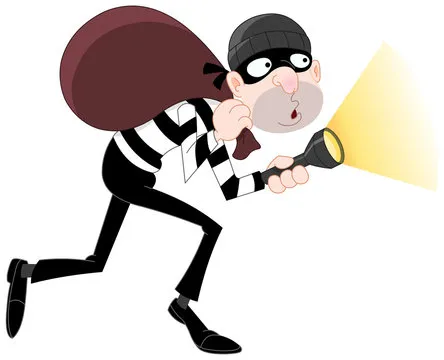
\includegraphics[width=\textwidth]{pic/thief.png} 
        
        \begin{tikzpicture}[remember picture,overlay]
        \node[anchor=south west, xshift=0.1cm, yshift=0.2cm] at (current page.south west) {
            \scriptsize Photo adapted from https://stock.adobe.com/search?k=thief+cartoon
        };
    \end{tikzpicture}
        
    \end{minipage}
    
\end{frame}

\begin{frame}{Performance metrics cont.}
    \begin{itemize}
        \item \textbf{Metrics:}
        \begin{itemize}
            % \item \textbf{Accuracy}:
            % \[
            % \text{Accuracy} = \frac{TP + TN}{TP + TN + FP + FN}
            % \]
            % \textit{Measures the overall correctness of the alarm system. It is the proportion of true results (both true positives and true negatives) among the total cases examined.}
            
            \item \textbf{Sensitivity (Recall)}:
            \[
            \text{Sensitivity} = \frac{TP}{TP + FN}
            \]
            \textit{Indicates the ability of the alarm system to correctly identify a thief. It is the proportion of actual positives (thief present) that are correctly identified.}

            \item \textbf{Specificity}:
            \[
            \text{Specificity} = \frac{TN}{TN + FP}
            \]
            \textit{Measures the ability of the alarm system to correctly identify when no thief is present. It is the proportion of actual negatives that are correctly identified.}

            \item \textbf{Precision}:
            \[
            \text{Precision} = \frac{TP}{TP + FP}
            \]
            \textit{Indicates the accuracy of the alarm when it rings. It is the proportion of times the alarm rang and a thief was indeed present out of all the times the alarm was activated.}
        \end{itemize}
    \end{itemize}
\end{frame}



%%%%%%%%%%%%%%%%%%%%%%%%%%%%%%%%%%%%%%%%%%%%%%%%%
% \begin{frame}{Performance metrics}
    
    
%     \begin{table}[h!]
%     \centering
%     \begin{tabular}{|c|c|c|}
%         \hline
%          & actually in the class & actually not in the  class \\ \hline
%         predicted to be in the class & TP & FP \\ \hline
%         predicted not to be in the class & FN & TN \\ \hline
%         % Row 3, Col 1 & Row 3, Col 2 & Row 3, Col 3 \\ \hline
%     \end{tabular}
%     % \caption{Basic Table}
%     % \label{tab:basic_table}
%     \end{table}
    
    
%     \begin{align*}
%         \text{Precision P } &= \frac{TP}{TP + FP} \\
%         \text{Recall R } &= \frac{TP}{TP + FN} \\
%         \text{Accuracy } &= \frac{TP + TN}{TP + TN + FP + FN}
%     \end{align*}
% \end{frame}
%%%%%%%%%%%%%%%%%%%%%%%%%%%%%%%%%%%%%%%%%%%%%%

%%%%%%%%%%%%%%%%%%%%%%%%%%%%%%%%%%%%%%%%%%%%%%
\begin{frame}{Performance metrics cont.}
    \begin{figure}[h]
            \centering
            
            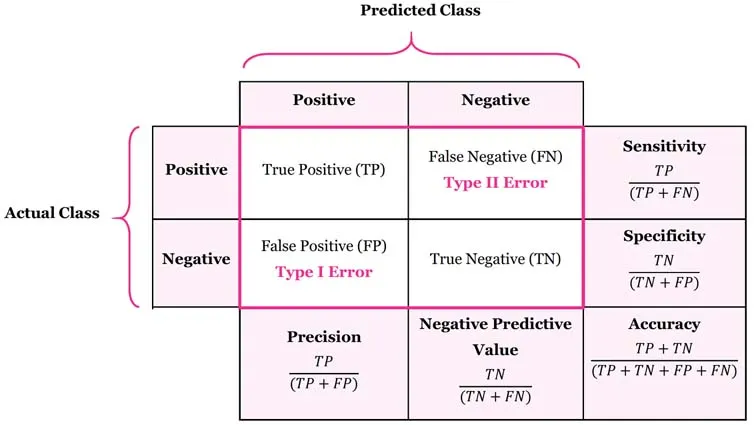
\includegraphics[width=0.8\textwidth]{pic/image.png}
            % \caption* { \scriptsize Figure adapted from }
            % \label{fig:image1}
            \end{figure}
            
    \vfill 
    
    \begin{tikzpicture}[remember picture,overlay]
        \node[anchor=south west, xshift=0.01cm, yshift=0.15cm] at (current page.south west) {
            \scriptsize Figure adapted from https://medium.com

        };
    \end{tikzpicture}
\end{frame}
%%%%%%%%%%%%%%%%%%%%%%%%%%%%%%%%%%%%%%%%%%%%%%
\begin{frame}{A combined measure: F1}
    \begin{itemize}
        \item Combined measure: \textbf{F1 measure}
        \begin{itemize}
            \item allows us to trade off precision and recall
            \item Provides a single measure balancing precision and recall.
            \item Useful in imbalanced datasets or when both types of error are significant.
            \item Trade-off: Increasing recall typically decreases precision and vice versa.
            \item harmonic mean of P and R:
        \end{itemize}
    \end{itemize}
    
    \begin{align*}
        \frac{1}{F}=\frac{1}{2}(\frac{1}{P}+\frac{1}{R})\newline
        \Rightarrow F = \frac{1}{\frac{1}{2P} + \frac{1}{2R}} = \frac{2PR}{P + R}
    \end{align*}
    % \[
    %     \hspace{10cm} \text{You can see: } \beta^2 = \frac{1-\alpha}{\alpha}
    % \]
    
    % \begin{itemize}
    %     \item Harmonic mean of P and R: 
    % \end{itemize}
    %     \begin{align*}
    %     \frac{1}{F}=\frac{1}{2}(\frac{1}{P}+\frac{1}{R})
    % \end{align*}
\end{frame}
%%%%%%%%%%%%%%%%%%%%%%%%%%%%%%%%%%%%%%%%%%%%%
% \begin{frame}{A combined measure: F1 cont.}
%     \begin{itemize}
%         \item People usually use balanced $F$ $(\beta=1 \text{ or } \alpha=\frac{1}{2})$
%     \end{itemize}
%     \begin{align*}
%         F &= F_{\beta=1} \\
%         &\\
%         F &= \frac{2PR}{P + R}
%     \end{align*}
%     \begin{itemize}
%         \item Harmonic mean of P and R: 
%     \end{itemize}
%     \begin{align*}
%         \frac{1}{F}=\frac{1}{2}(\frac{1}{P}+\frac{1}{R})
%     \end{align*}
% \end{frame}
%%%%%%%%%%%%%%%%%%%%%%%%%%%%%%%%%%%%%%%%%%%%%%
\begin{frame}{Precision/recall/F1}
    \begin{itemize}
        \item This website could give you a perfect intuition about precision recall trade-off
        
    \end{itemize}
    \begin{figure}[h]
            \centering
            
            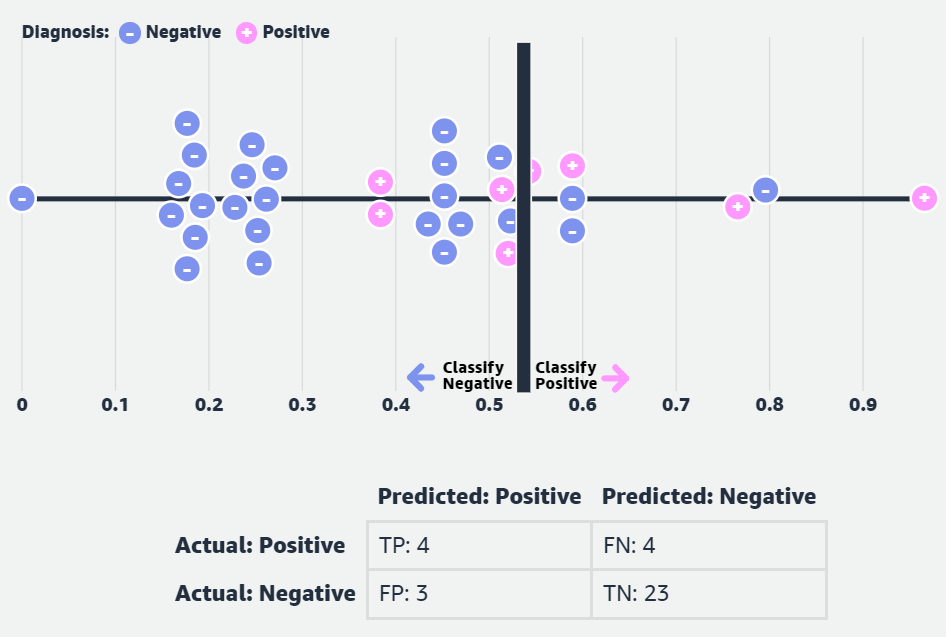
\includegraphics[width=0.5\textwidth]{pic/prRtradeoff.png}
            % \caption* { \scriptsize [}
            % \label{fig:image1}
            \end{figure}
    \begin{itemize}
        \item Link: \href{https://mlu-explain.github.io/precision-recall/}{https://mlu-explain.github.io/precision-recall/}
    \end{itemize}
\end{frame}
%%%%%%%%%%%%%%%%%%%%%%%%%%%%%%%%%%%%%%%%%%%%%%
\begin{frame}{Why harmonic mean?}
    \begin{itemize}
        \item Why don't we use a different mean of P and R as a measure?
        \begin{itemize}
            \item e.g., the arithmetic mean
        \end{itemize}
        \item The simple (arithmetic) mean is $50\%$ for "return true for every thing", which is too high.
        \item Desideratum: Punch really bad performance either on precision or recall
        \begin{itemize}
            \item Taking the minimum achieves this.
            \item F (harmonic mean) is a kind of \textbf{smooth minimum}.
        \end{itemize}
    \end{itemize}
\end{frame}
%%%%%%%%%%%%%%%%%%%%%%%%%%%%%%%%%%%%%%%%%%%%%%
\begin{frame}{F1 and other averages}
    \begin{itemize}
        \item Harmonic mean is a conservative average. We can view the harmonic mean as a kind of soft minimum
    \end{itemize}
    
    \begin{figure}[h]
            \centering
            
            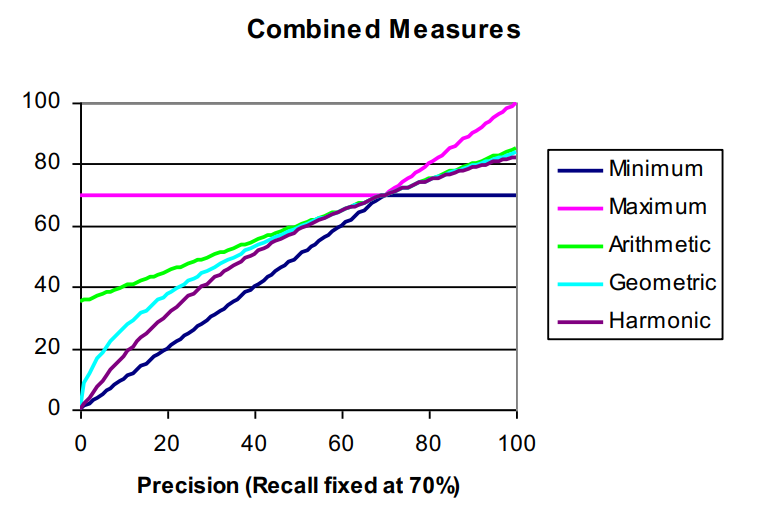
\includegraphics[width=0.58\textwidth]{pic/F1andOthers.png}
            % \caption* { \scriptsize [}
            % \label{fig:image1}
            \end{figure}
    
    \vfill 
    
    \begin{tikzpicture}[remember picture,overlay]
        \node[anchor=south west, xshift=0.01cm, yshift=0.15cm] at (current page.south west) {
            \scriptsize Figure adapted from M.Soleymani ML slides, Sharif University of Technology
        };
    \end{tikzpicture}
\end{frame}

\begin{frame}{Comparative Overview}
    \begin{center}
    \begin{tabular}{lccc}
        \toprule
        Metric & Formula & Focus & Typical Use-Case \\
        \midrule
        Accuracy & $\frac{TP+TN}{TP+FP+FN+TN}$ & Overall correctness & Balanced classes \\
        Precision & $\frac{TP}{TP+FP}$ & False positive control & Spam detection, IR \\
        Recall & $\frac{TP}{TP+FN}$ & False negative control & Medical diagnosis, anomaly detection \\
        F1-Score & $2\frac{PR}{P+R}$ & Balance & Imbalanced or skewed datasets \\
        \bottomrule
    \end{tabular}
    \end{center}
    \vspace{0.3cm}
    \begin{itemize}
        \item Metric choice should reflect operational objectives and misclassification costs.
        \item Always interpret metrics in conjunction with the confusion matrix.
    \end{itemize}
\end{frame}
%%%%%%%%%%%%%%%%%%%%%%%%%%%%%%%%%%%%%%%%%%%%%%
% \begin{frame}{A precision-recall curve}
%     \begin{figure}[h]
%             \centering
            
%             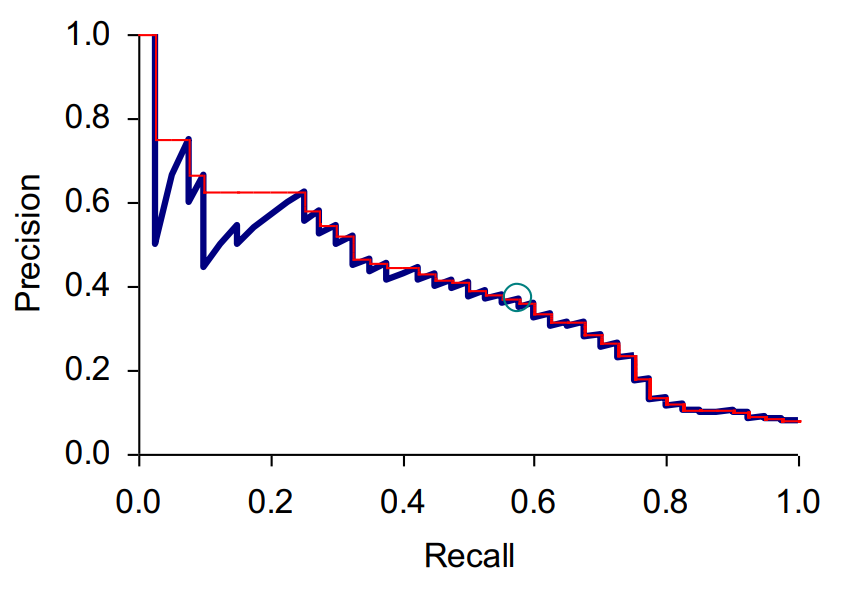
\includegraphics[width=0.68\textwidth]{pic/preReCurv.png}
%             % \caption* { \scriptsize [}
%             % \label{fig:image1}
%             \end{figure}
% \end{frame}
%%%%%%%%%%%%%%%%%%%%%%%%%%%%%%

%%%%%%%%%%%%%%%%%%%%%%%%%%%%
\begin{frame}{Confusion matrix}
    \begin{itemize}
        \item The \textbf{confusion matrix} is a \textbf{table} used to evaluate the performance of a classification model.
        \item It compares the \textbf{actual values (true labels)} with the \textbf{predicted values} from the model.
        \item Each \textbf{row} of the matrix represents the \textbf{actual class}, while each \textbf{column} represents the \textbf{predicted class}.
        \item It helps us understand not just how often the model is correct, but also \textbf{where it makes mistakes}.
    \end{itemize}
    
    % \vfill
    % \centering
    % \includegraphics[width=0.5\textwidth]{confusion_matrix_image.png}
    % % Add an illustrative image of a confusion matrix
\end{frame}


%%%%%%
\begin{frame}{Confusion matrix cont.}
    \begin{itemize}
        \item Let's consider an image classification task where we classify images into three categories: **Cat**, **Dog**, and **Horse**.
        \item After training the model, we evaluate its predictions against the actual labels.
    \end{itemize}
    
    \vfill
    \centering
    \begin{tabular}{|c|c|c|c|}
    \hline
    & \textbf{Predicted Cat} & \textbf{Predicted Dog} & \textbf{Predicted Horse} \\
    \hline
    \textbf{Actual Cat} & True Positive (TP) & False Negative (FN) & False Negative (FN) \\
    \hline
    \textbf{Actual Dog} & False Negative (FN) & True Positive (TP) & False Negative (FN) \\
    \hline
    \textbf{Actual Horse} & False Negative (FN) & False Negative (FN) & True Positive (TP) \\
    \hline
    \end{tabular}
\end{frame}

%%%%%%%
\begin{frame}{Confusion matrix cont.}
    \begin{minipage}{0.4\textwidth}
        \begin{itemize}
            \item Here is an example confusion matrix for a model that classifies images of cats, dogs, and horses:
            \item We can see that the model classified 8 images of cats correctly, but it classified 1 cat as a dog and 1 cat as a horse (False Negatives).
            \item Similarly, it made 2 mistakes when predicting dogs and horses.
        \end{itemize}
    \end{minipage}
    \hfill
    \begin{minipage}{0.55\textwidth}
        \begin{figure}[h]
            \centering
            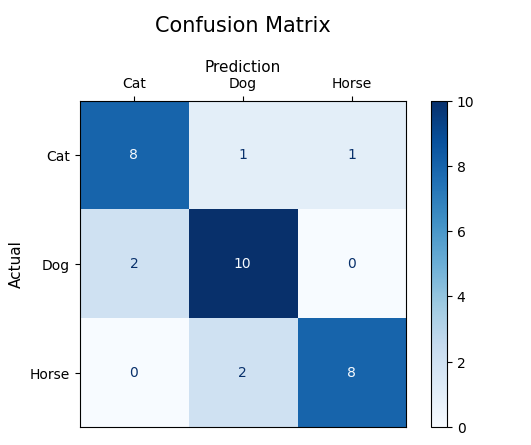
\includegraphics[width=1\textwidth]{pic/cmCatDogHorse.png}
            \caption* {\scriptsize Figure adapted from https://www.geeksforgeek}
        \end{figure}
    \end{minipage}
\end{frame}


%%%%%%%%%%%%%%%%%%%%%%%%%%%%%%
% \begin{frame}{Confusion matrix}
%     \begin{itemize}
%         \item This  $(i,j)$ entry means $53$ of the samples actually in class $i$ were put in class $j$ by the classifier:
%     \end{itemize}
%     \begin{figure}[h]
%             \centering
            
%             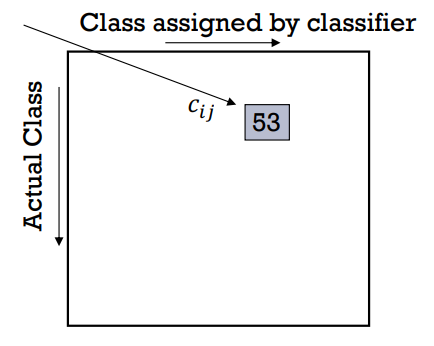
\includegraphics[width=0.4\textwidth]{pic/cmatrix.png}
%             % \caption* { \scriptsize [}
%             % \label{fig:image1}
%             \end{figure}
%     \begin{itemize}
%         \item In a perfect classification, only the diagonal has non-zero entries
%     \end{itemize}
% \end{frame}
%%%%%%%%%%%%%%%%%%%%%%%%%%%%%%%%%%%%%%%%%%%
\begin{frame}{Per class evaluation measures}
    \begin{itemize}
        \item \textbf{Definition:} For our \textbf{confusion matrix} $\mathbf{C}$, each \textbf{element} $\mathbf{C_{ij}}$ denotes the number of samples actually in class $i$ that were put in class $j$ by our classifier.
        \begin{itemize}
            \item Now we could rewrite our performance metrics with confusion matrix view
        \end{itemize}
        \noindent\hrulefill 
        \item Recall: Fraction of the samples in class $i$ classified correctly:
        \[
          \frac{C_{ii}}{\sum _{j} C_{ij}}    
        \]
        \item Precision: Fraction of the samples assigned class $i$ that are actually about class $i$:
        \[
          \frac{C_{ii}}{\sum _{j} C_{ji}}
        \]
        \item Accuracy: Fraction of the samples classified correctly:
        \[
          \frac{\sum _i {C_{ii}}}{\sum _j \sum _i C_{ij}}
        \]
    \end{itemize}
    
\end{frame}
%%%%%%%%%%%%%%%%%%%%%%%%%%%%
\begin{frame}{Averaging: macro vs. micro}
    \begin{itemize}
        \item We now have an evaluation measure (F1) for one class.
        \item But we also want a single number that shows \textcolor{deepred}{aggregate performance} over all classes
    \end{itemize}
\end{frame}
%%%%%%%%%%%%%%%%%%%%%%%%%%%%
\begin{frame}{Micro- vs. Macro-Averaging}
    \begin{itemize}
        \item If we have more than one class, how do we combine
multiple performance measures into one quantity?
        \item \textcolor{deepred}{Macroaveraging}: Compute performance for each class, then average
        \begin{itemize}
            \item Compute F1 for each of the $C$ classes
            \item Average these $C$ numbers
        \end{itemize}
        \item \textcolor{deepred}{Microaveraging}: Collect decisions for all classes, aggregate them and then compute measure.
        \begin{itemize}
            \item Compute TP, FP, FN for each of the $C$ classes.
            \item Sum these $C$ numbers(e.g, all TP to get aggregate TP)
            \item Compute F1 for aggregate TP, FP, FN
        \end{itemize}
    \end{itemize}
\end{frame}
%%%%%%%%%%%%%%%%%%%%%%%%%%%%
\begin{frame}{Micro- vs. Macro-Averaging: example}
    \begin{figure}[h]
            \centering
            
            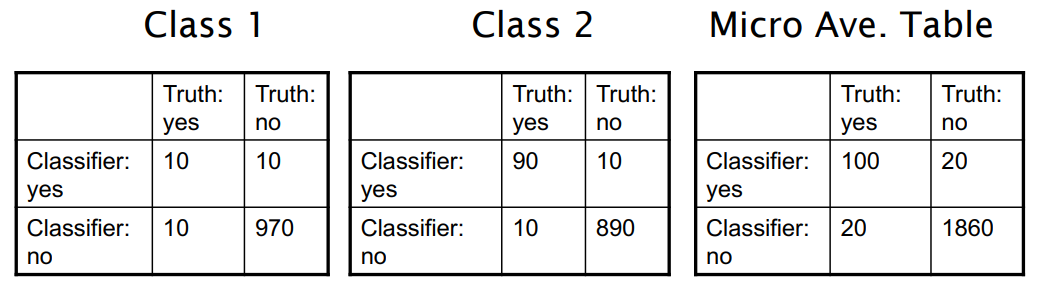
\includegraphics[width=0.8\textwidth]{pic/MicroVsMacro.png}
            % \caption* { \scriptsize [}
            % \label{fig:image1}
            \end{figure}
            
    \begin{itemize}
        \item Macroaveraged precision: $(0.5 + 0.9)/2 = 0.7$
        \item Microaveraged precision: $100/120 = 0.83$
        \item Microaveraged score is dominated by score on common classes
    \end{itemize}
\end{frame}
%%%%%%%%%%%%%%%%%%%%%%%%%%%
% \begin{frame}{Imbalanced classification}
%     \begin{itemize}
%         \item Accuracy is not a proper criteria
%         \item Micro-F1 for multi-class classification is equal to accuracy
%         \item Macro-F1 is more suitable for this purpose
%     \end{itemize}
% \end{frame}
%%%%%%%%%%%%%%%%%%%%%%%%%%%%%
\begin{frame}{AUC-ROC}
    \begin{itemize}
        \item Area Under the Receiver Operating Characteristic Curve
        \begin{itemize}
            \item ROC (Receiver Operating Characteristic) is a graphical representation of the performance of a binary classification model.
            \item It plots the true positive rate (TPR) against the false positive rate (FPR) at different classification thresholds.
        \end{itemize}
        
    \end{itemize}
    
    \begin{figure}[h]
            \centering
            
            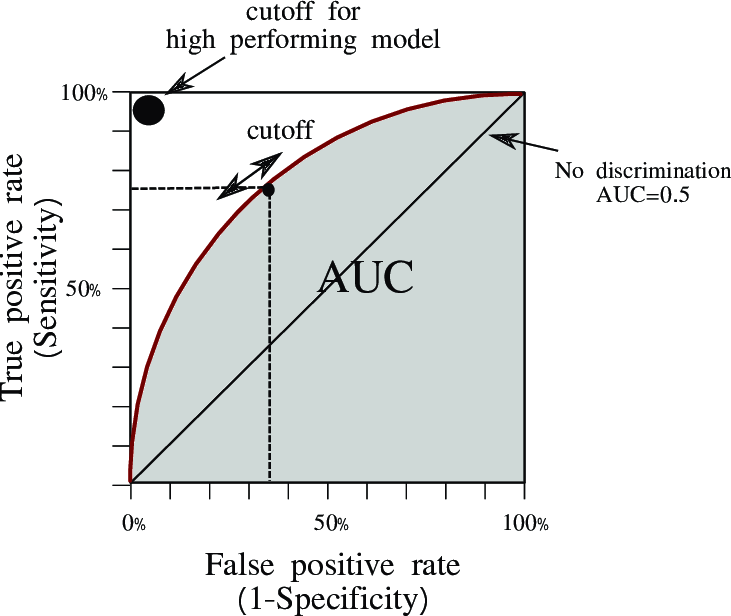
\includegraphics[width=0.4\textwidth]{pic/AUC.png}
            % \caption* { \scriptsize [}
            % \label{fig:image1}
            \end{figure}
    
    \vfill 
    
    \begin{tikzpicture}[remember picture,overlay]
        \node[anchor=south west, xshift=0.01cm, yshift=0.15cm] at (current page.south west) {
            \scriptsize Figure adapted from https://www.researchgate.net/figure/ROC-curves-and-area-under-curve-AUC_fig2_351506473

        };
    \end{tikzpicture}
    
\end{frame}

%%%%%%%%%%%%%%%%%%%%%%%%%%%
\begin{frame}{AUC-ROC cont.}
    \begin{itemize}
        \item A high AUC score indicates that the model has good discrimination ability, i.e., it can effectively differentiate between positive and negative instances at different classification thresholds.
        \item Conversely, a lower AUC-ROC score suggests that the model struggles to differentiate between the two classes.
        \item AUC ranges from 0 to 1, with 0.5 indicating random guessing and 1 indicating a perfect classifier.


    \end{itemize}
\end{frame}
%%%%%%%%%%%%%%%%%%%%%%%%%%%%


\section{Imbalanced Data}

\begin{frame}{The Problem: Imbalanced Data}
    \begin{itemize}\itemsep1em
        \item Real-world datasets often contain classes with unequal representation.
        \item \textbf{Examples:}
        \begin{itemize}
            \item Fraud detection: 0.1\% Fraud, 99.9\% Non-Fraud
            \item Medical diagnosis: 2\% Disease, 98\% Healthy
        \end{itemize}
        \item \textbf{Issue:} High accuracy may hide poor performance on the minority class.
    \end{itemize}
    \begin{center}
        \includegraphics[width=0.55\textwidth]{pic/figure_32.png}\\
    \end{center}
\end{frame}

\begin{frame}{Solution 1: Resampling Techniques}
    \begin{columns}[T]
        \begin{column}{0.48\textwidth}
            \textbf{Undersampling}
            \begin{itemize}\itemsep0.8em
                \item Remove samples from majority class.
                \item \textbf{+} Reduces training time.
                \item \textbf{--} Risk of losing information.
            \end{itemize}
            \vspace{0.8em}
            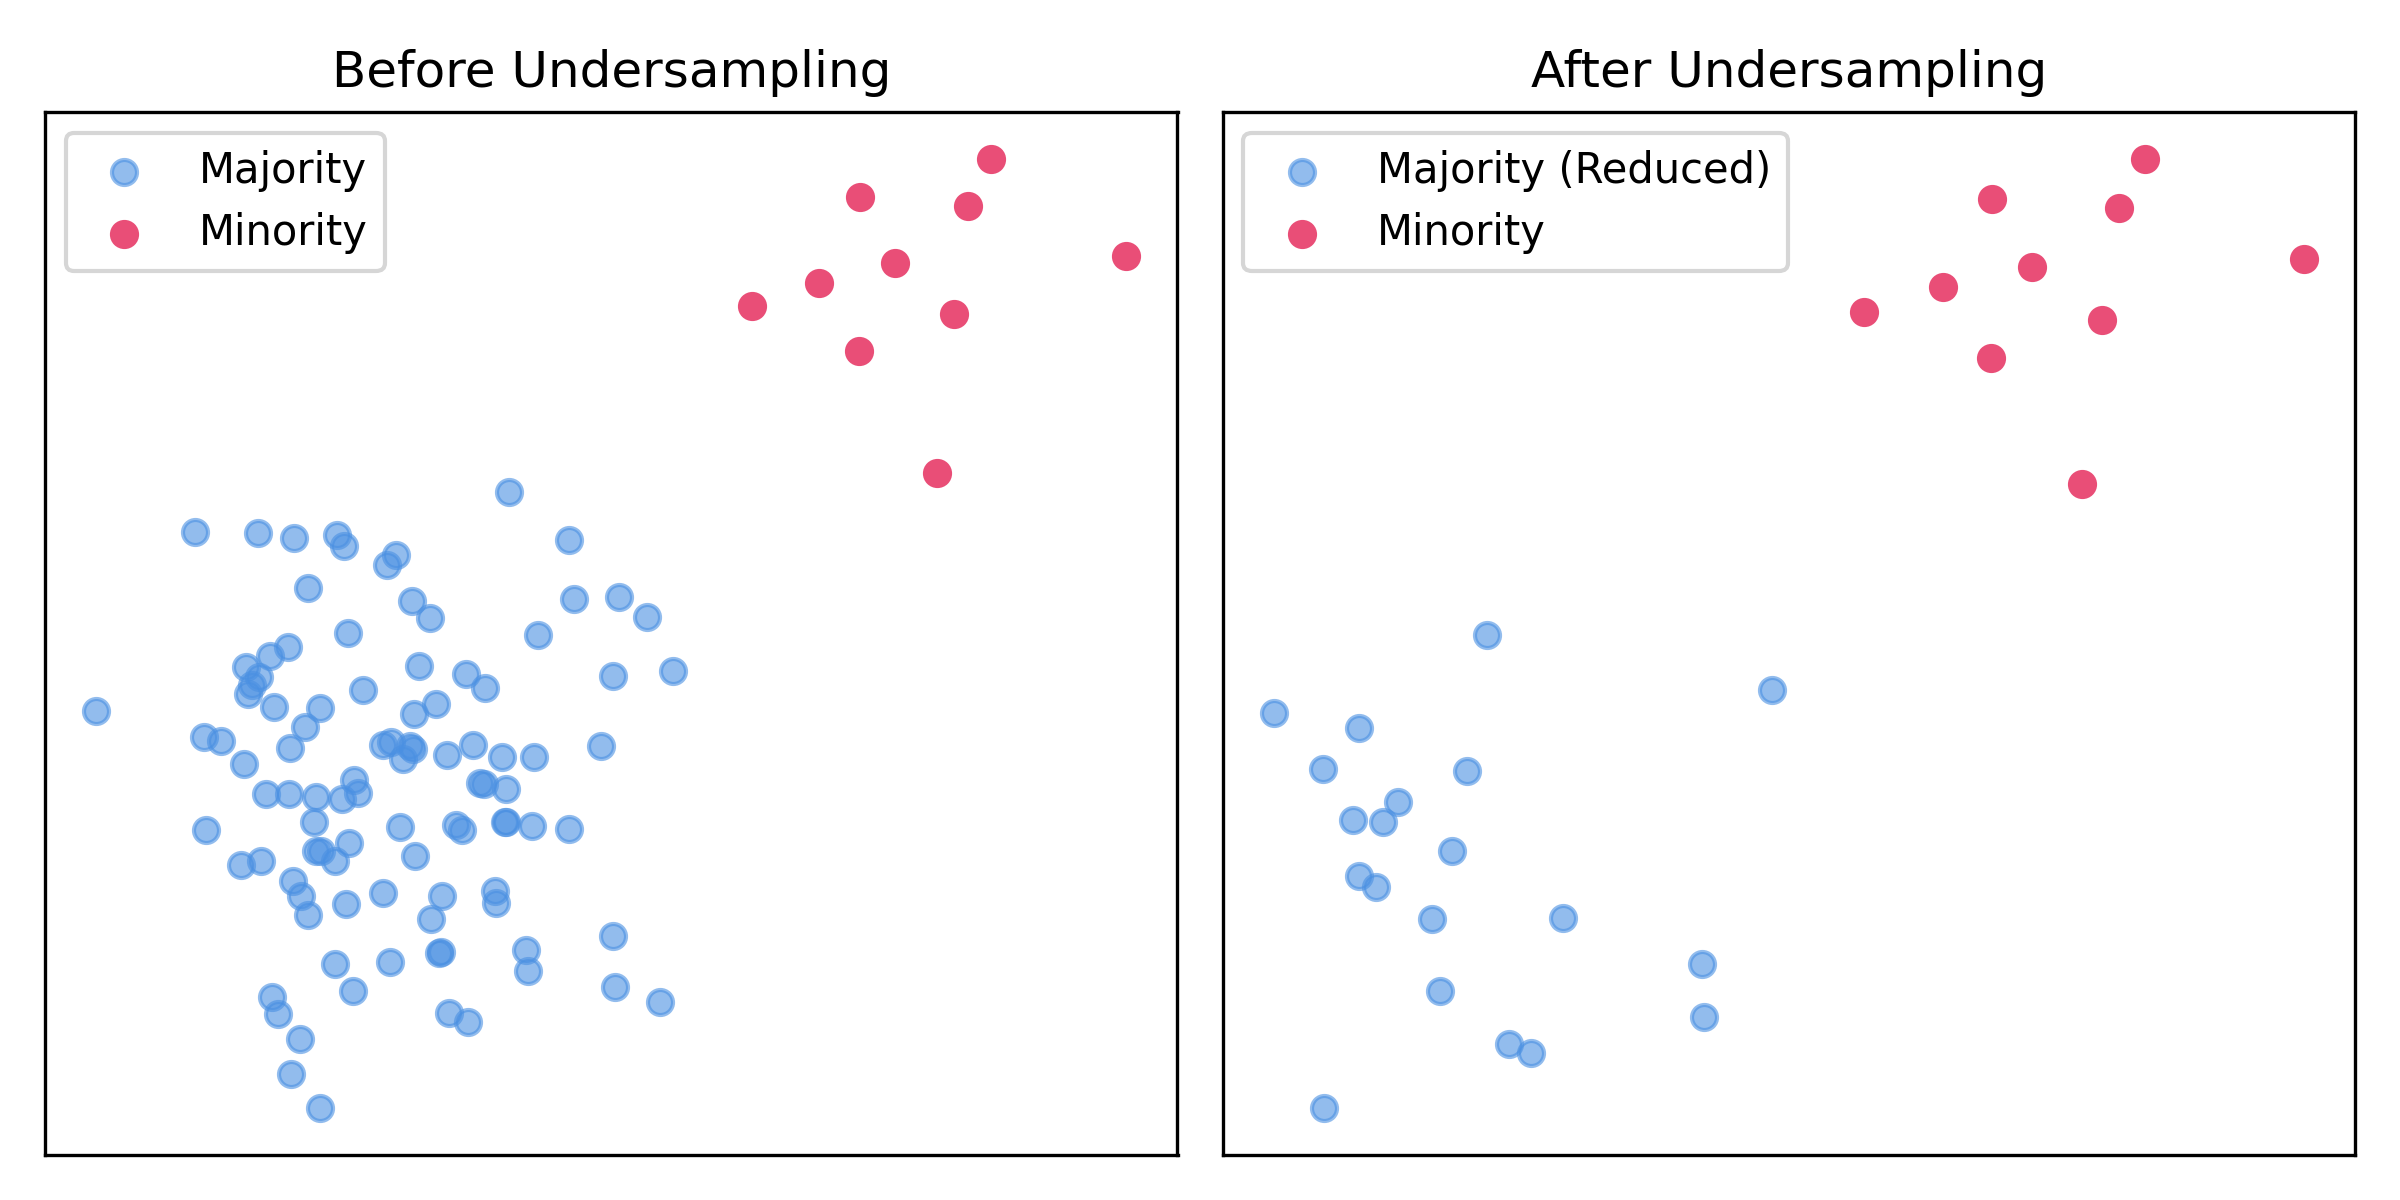
\includegraphics[width=\textwidth]{pic/Figure_33.png}\\
            \scriptsize Majority class reduced.
        \end{column}

        \begin{column}{0.48\textwidth}
            \textbf{Oversampling (e.g., SMOTE)}
            \begin{itemize}\itemsep0.8em
                \item Generate synthetic minority samples.
                \item \textbf{+} Preserves information.
                \item \textbf{--} May cause overfitting.
            \end{itemize}
            \vspace{0.8em}
            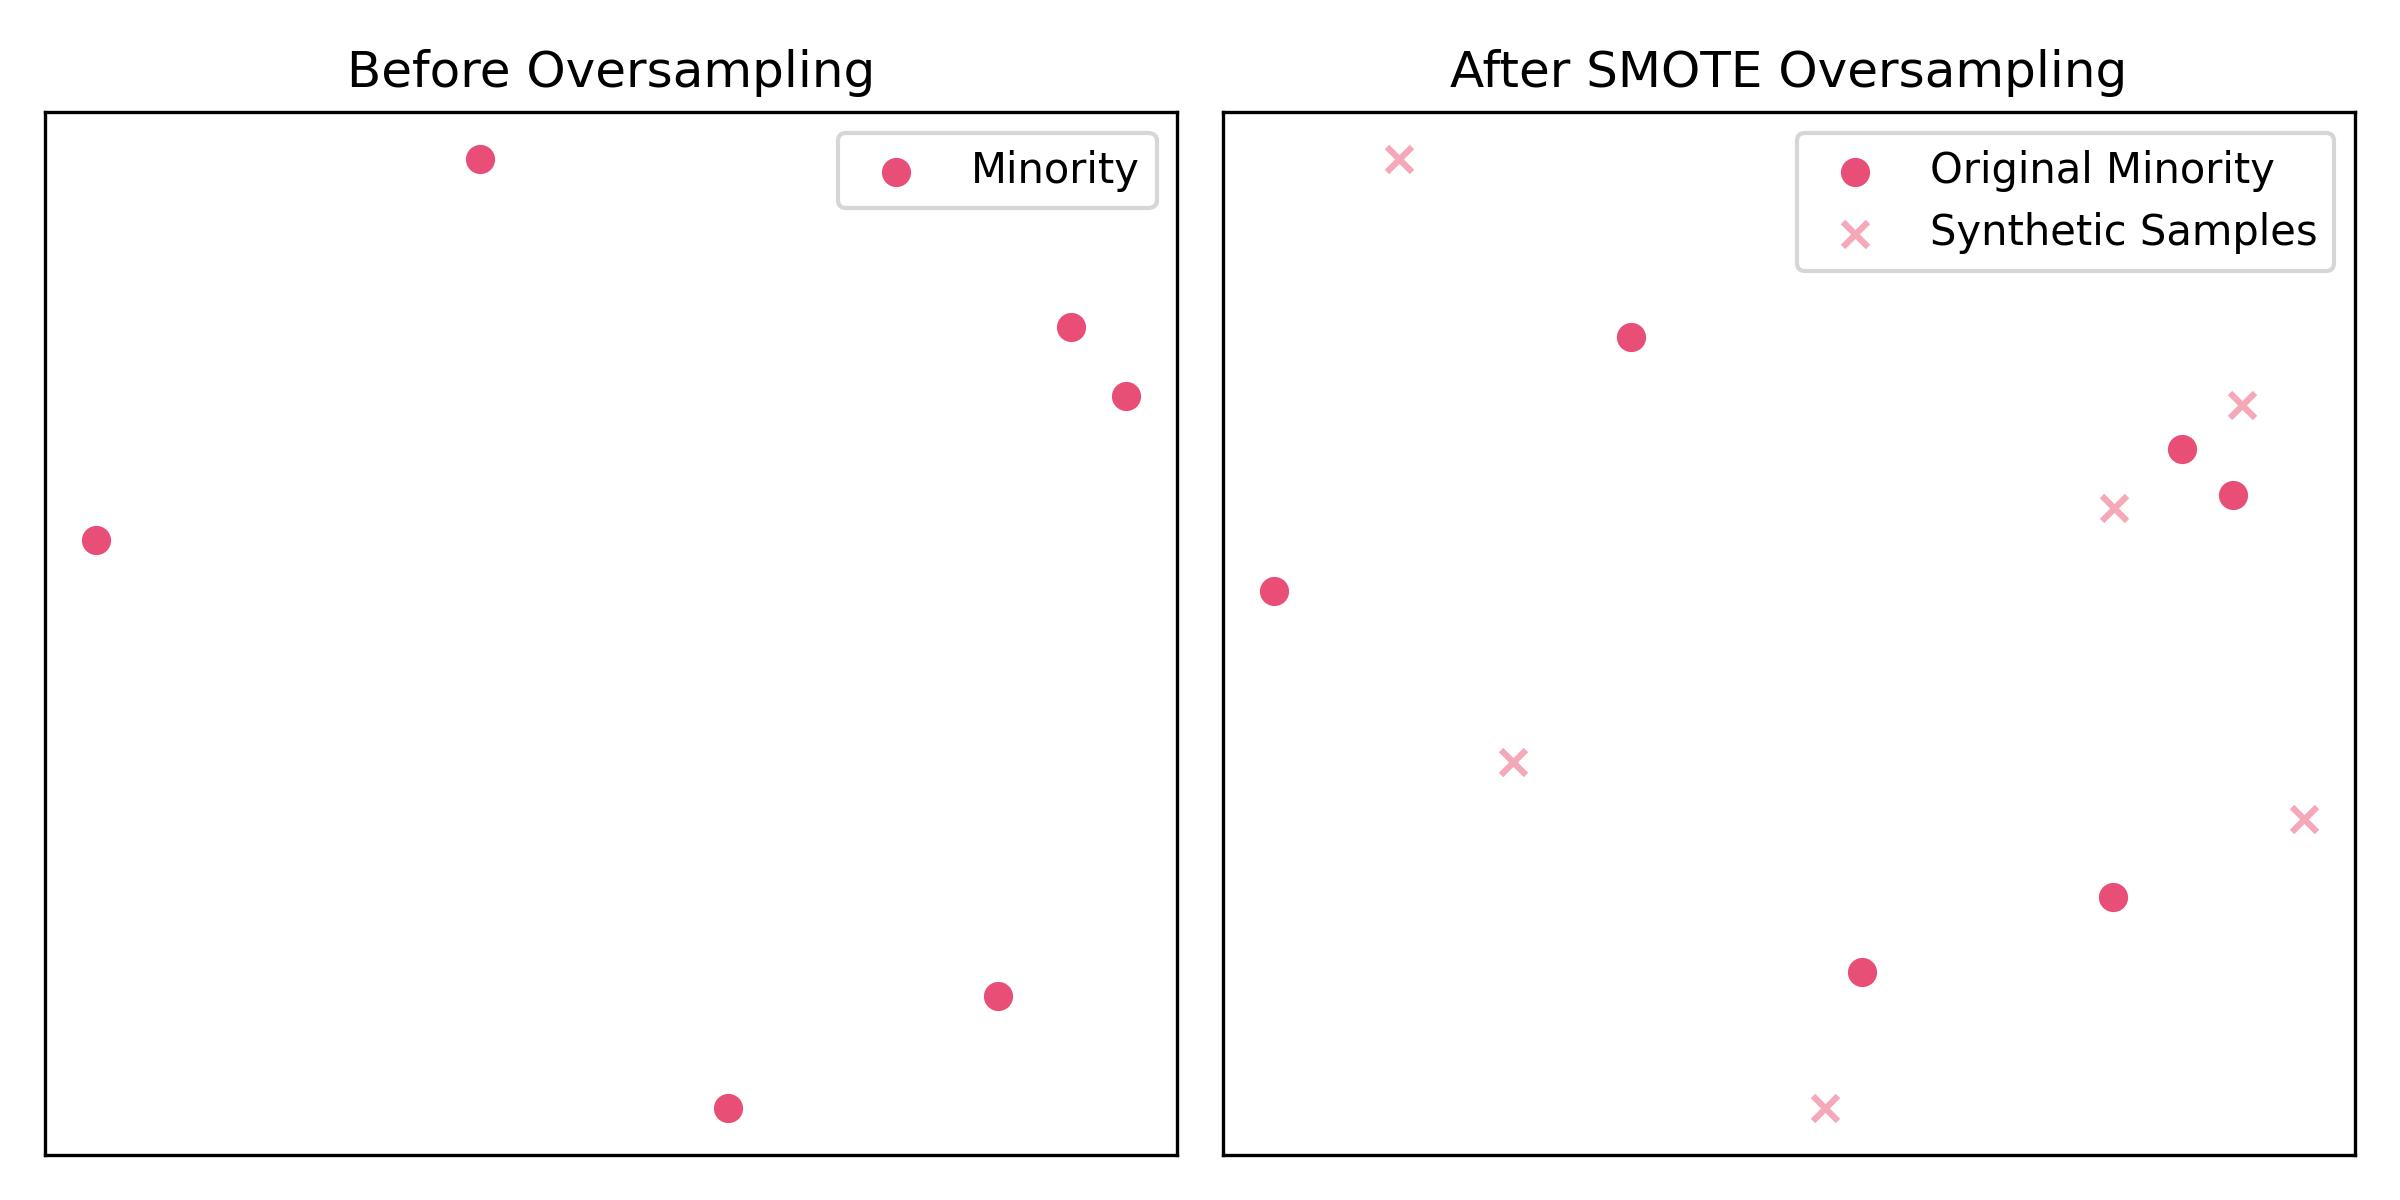
\includegraphics[width=\textwidth]{pic/Figure_34.png}\\
            \scriptsize New minority points added via interpolation.
        \end{column}
    \end{columns}
\end{frame}

\begin{frame}{Solution 2: Algorithmic Approaches}

\textbf{Weighted Loss Function}

\begin{itemize}\itemsep0.8em
    \item Assign a higher penalty to errors on the minority class.
    \item Encourages the model to focus on rare but important cases.
\end{itemize}

\vspace{0.5em}

\begin{columns}[c,onlytextwidth]
    \column{0.55\textwidth}
    \[
        J(w) = - \sum_{i} w_{y^{(i)}} \, y^{(i)} \log(\hat{y}^{(i)})
    \]
    \scriptsize
    \begin{center}
    where $w_{y^{(i)}}$ is larger for the minority class.
    \end{center}

    \column{0.45\textwidth}
    \centering
    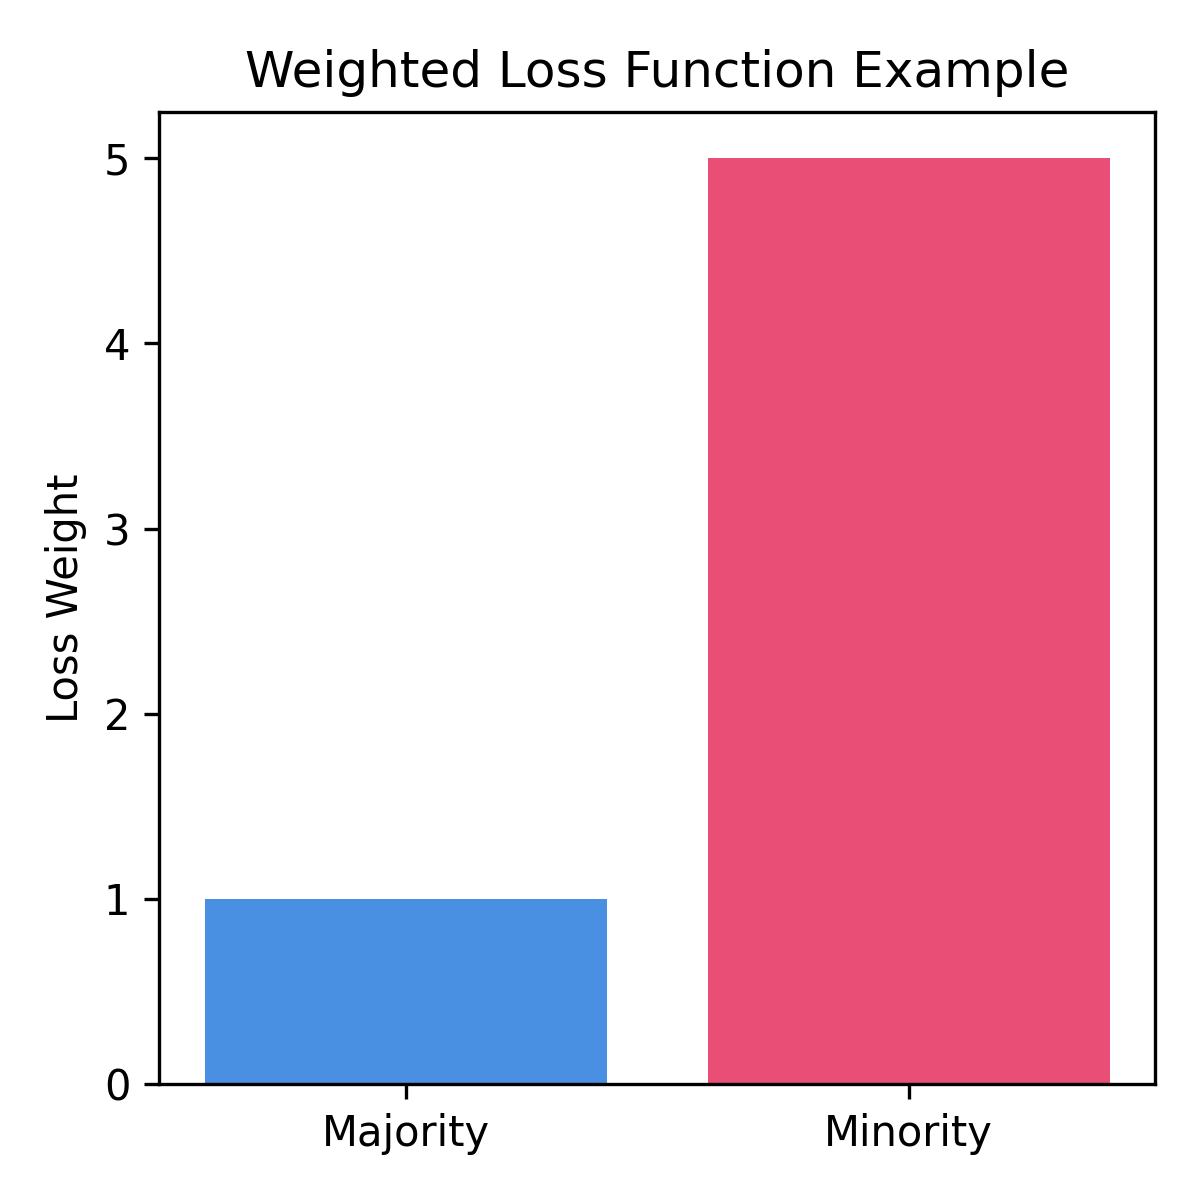
\includegraphics[width=0.8\linewidth]{pic/Figure_36.png}\\
\end{columns}

\end{frame}



\begin{frame}{Hybrid Approaches}

\textbf{Combining Sampling Strategies}

\begin{itemize}\itemsep0.8em
    \item Integrates both oversampling and undersampling to achieve better class balance.
\end{itemize}

\vspace{0.5em}

\textbf{Typical Pipeline:}
\begin{enumerate}\itemsep0.6em
    \item Apply \textbf{SMOTE} to synthetically augment minority samples.
    \item Randomly undersample the majority class to reduce imbalance.
    \item Train the model on the newly balanced dataset.
\end{enumerate}

\vspace{0.6em}

\begin{itemize}\itemsep0.6em
    \item Provides a practical trade-off between \textbf{bias} and \textbf{variance}.
\end{itemize}

\end{frame}


\begin{frame}{Comparison of Methods}

\begin{columns}[c,onlytextwidth]
    \column{0.55\textwidth}
    \textbf{Summary}

    \begin{itemize}\itemsep0.6em
        \item \textbf{Sampling} — modifies data distribution\\
        \textcolor{green!60!black}{\small(+ Simple, improves balance)}\\
        \textcolor{red!70!black}{\small(– Risk of over/underfitting)}
        
        \item \textbf{Algorithmic} — adjusts model focus  \\
        \textcolor{green!60!black}{\small(+ No data change, interpretable)}\\
        \textcolor{red!70!black}{\small(– Needs careful weight tuning)}
        
        \item \textbf{Hybrid} — combines both strategies  \\
        \textcolor{green!60!black}{\small(+ Balanced, strong results)}  \\
        \textcolor{red!70!black}{\small(– More complex, slower training)}
    \end{itemize}

    \column{0.43\textwidth}
    \centering
    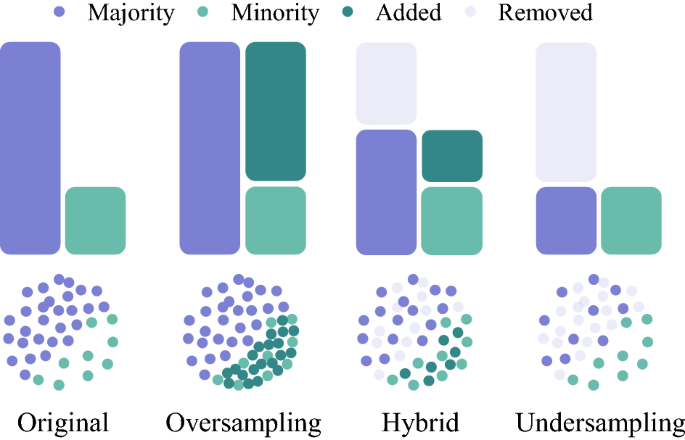
\includegraphics[width=0.9\linewidth]{pic/Figure_35.png}\\
    \scriptsize Visual summary of trade-offs
\end{columns}

\end{frame}





\section{Cross Validation}

\begin{frame}{Model Selection via Cross Validation}
    \begin{itemize}
        \item \textbf{Cross-Validation}
        \medskip
        \begin{itemize}\itemsep1em
            \item \justifying \textbf{Purpose}:
            Technique for evaluating how well a model generalizes to unseen data.
            \item \justifying \textbf{How It Works}:
            Split data into $k$ folds; train on $k-1$ folds and validate on the remaining fold.
            \item \justifying \textbf{Repeat Process}:
            Repeat $k$ times, rotating the test fold each time. Average of all scores is the final score of the model.
            \item \justifying Cross-validation
            reduces overfitting and provides a more reliable estimation of model performance.
        \end{itemize}
    \end{itemize}
\end{frame}


\begin{frame}{K-Fold Cross Validation}
    \begin{figure}
        \centering
        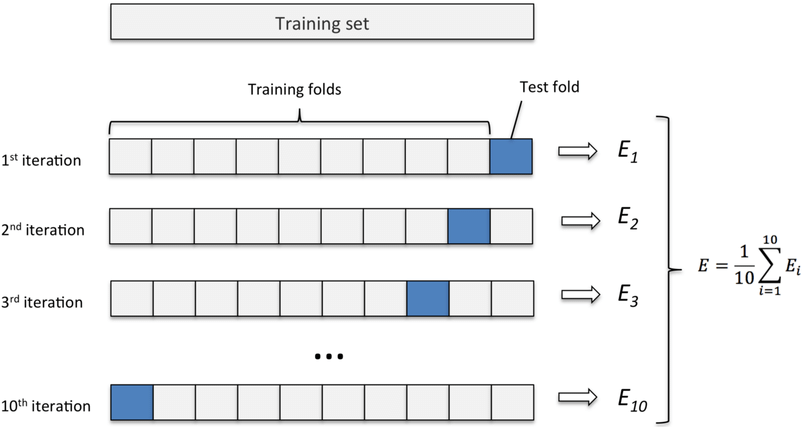
\includegraphics[width=.8\textwidth]{pic/Figure_28.png}
    \end{figure}
    \vfill
    \begin{tikzpicture}[remember picture,overlay]
        \node[anchor=south west, xshift=0.1cm, yshift=0.22cm] at (current page.south west) {
            \scriptsize Figure adapted from Introduction to Support Vector Machines and Kernel Methods, J.M. Ashfaque.
        };
    \end{tikzpicture}
\end{frame}


\begin{frame}{Leave-One-Out Cross-Validation (LOOCV)}
    \begin{itemize}
        \item \textbf{Leave-One-Out Cross-Validation (LOOCV)}
            \medskip
            \begin{itemize}\itemsep1em
            \item \justifying \textbf{How It Works}:
            Uses a single data point as the validation set ($k$ = 1) and the rest as the training set. Repeat for all data points.
            \item \textbf{Properties:}
            \smallskip
            \begin{itemize}\itemsep.5em
                \item \textbf{No Data Wastage}:
                Every data point is used for both training and validation.
                \item \textbf{High Variance, Low Bias}.
                \item \justifying \textbf{Computationally Expensive}: 
                Requires training the model $N$ times for $N$ data points, making it slow for large datasets.
                \item \textbf{Best for small datasets}.
            \end{itemize}
        \end{itemize}
    \end{itemize}
\end{frame}

\begin{frame}{Cross-Validation for Choosing Regularization Term}
    \begin{figure}
        \centering
        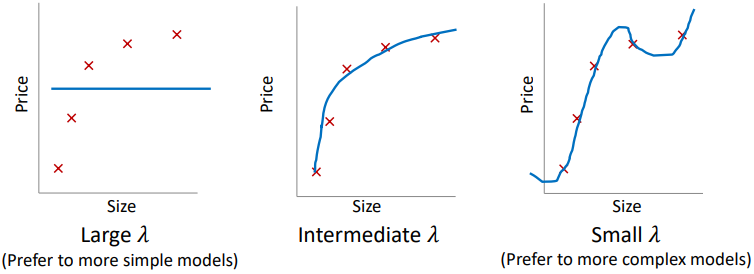
\includegraphics[width=0.8\linewidth]{pic/Figure_29.png}
    \end{figure}
    \vfill
    \begin{tikzpicture}[remember picture,overlay]
        \node[anchor=south west, xshift=0.1cm, yshift=0.22cm] at (current page.south west) {
            \scriptsize Figures adapted from slides of F.Salehi, Machine Learning course, Sharif University of Technology.
        };
    \end{tikzpicture}
\end{frame}

\begin{frame}{Cross-Validation for Choosing Model Complexity}
    \begin{figure}
        \centering
        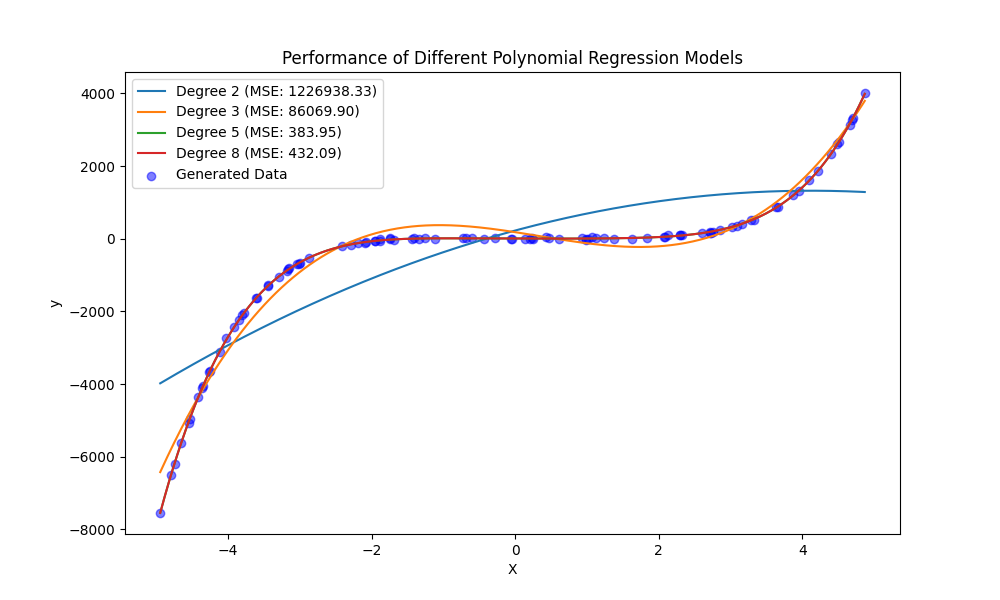
\includegraphics[width=0.8\linewidth]{pic/Figure_16.png}
    \end{figure}
\end{frame}



\begin{frame}[allowframebreaks]
    \bibliography{ref}
    \bibliographystyle{ieeetr}
    \nocite{*} % used here because no citation happens in slides
    % if there are too many try use:
    % \tiny\bibliographystyle{alpha}
\end{frame}

\end{document}